\documentclass[a4paper,14pt]{article}

\usepackage{comment} % Para comentar várias linhas ao mesmo tempo

%matemática
\usepackage{amsmath}
\usepackage{amssymb}

%diagramação
\usepackage{extsizes}
\everymath{\displaystyle}
\usepackage{geometry}
\usepackage{fancyhdr}
\usepackage{multicol}
\usepackage{graphicx}
\usepackage[brazil]{babel}
\usepackage[shortlabels]{enumitem}
\usepackage{cancel}
\usepackage{textcomp}
\usepackage{tcolorbox}

%tabelas
\usepackage{array} % Para melhor formatação de tabelas
\usepackage{longtable}
\usepackage{booktabs}  % Para linhas horizontais mais bonitas
\usepackage{float}   % Para usar o modificador [H]
\usepackage{caption} % Para usar legendas em tabelas
\usepackage{wrapfig} % Para usar tabelas e figuras flutuantes


%tikzpicture
\usepackage{tikz}
\usepackage{scalerel}
\usepackage{pict2e}
\usepackage{tkz-euclide}
\usetikzlibrary{calc}
\usetikzlibrary{patterns,arrows.meta}
\usetikzlibrary{shadows}
\usetikzlibrary{external}


%pgfplots
\usepackage{pgfplots}
\pgfplotsset{compat=newest}
\usepgfplotslibrary{statistics}
\usepgfplotslibrary{fillbetween}

%colours
\usepackage{xcolor}



\columnsep=2cm
\hoffset=0cm
\textwidth=8cm
\setlength{\columnseprule}{.1pt}
\setlength{\columnsep}{2cm}
\renewcommand{\headrulewidth}{0pt}
\geometry{top=1in, bottom=1in, left=0.7in, right=0.5in}

\pagestyle{fancy}
\fancyhf{}
\fancyfoot[C]{\thepage}

\begin{document}
	
	\noindent\textbf{6FMA28 - Matemática} 
	
	\begin{center}Perímetro (Versão estudante)
	\end{center}
	
	\noindent\textbf{Nome:} \underline{\hspace{10cm}}
	\noindent\textbf{Data:} \underline{\hspace{4cm}}
	
	%\section*{Questões de Matemática}
	
	\begin{multicols}{2}
		\noindent Perímetro é o comprimento da linha que contorna ou limita uma figura ou região plana. \\
		O perímetro de uma figura plana formada por segmentos de reta é igual à soma das medidas desses segmentos. \\
		No caso de uma circunferência, há uma estimativa que podemos usar para calcular seu perímetro: basta multiplicar o seu diâmetro por 3.
		\\
		\noindent\textsubscript{-----------------------------------------------------------------------}
		\begin{enumerate} 
			\item Uma pessoa tem vários animais e deseja mantê-los em um terreno que comprou. O terreno tem a forma de um retângulo com 42 m de comprimento por 21 de largura. Cada metro de cerca custa 18 reais. Quanto essa pessoa irá gastar para cercar todo o terreno? \\ 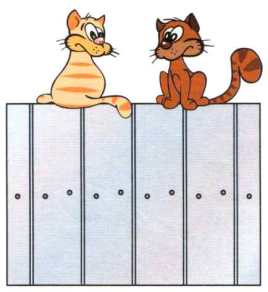
\includegraphics[width=1\linewidth]{6FMA28_imagens/imagem1} \\
			\item Qual é o perímetro do jardim cuja planta está representada abaixo? \\
			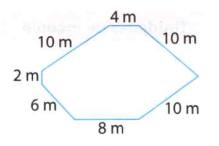
\includegraphics[width=1\linewidth]{6FMA28_imagens/imagem2} \\\\\\\\
			\item Qual é o comprimento, em centímetros, da linha representada abaixo? \\
			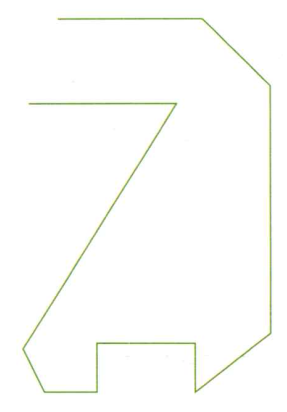
\includegraphics[width=1\linewidth]{6FMA28_imagens/imagem3}
			\item Uma praça circular tem um raio de 20 metros e deve ser cercada. Faça uma estimativa do comprimento dessa cerca. \\\\\\\\\\\\\\\\\\\\
			%99 a 101
			\item Na figura abaixo está representada a planta de um terreno. Qual é o seu perímetro, em metros? \\
			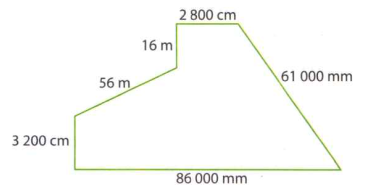
\includegraphics[width=1\linewidth]{6FMA28_imagens/imagem4} \\\\\\\\\\\\\\\\\\\\
			\item Um empresário comprou um lote de terra cuja forma é um retângulo de 82 m de comprimento por 63 m de largura. Ele quer contornar o terreno com uma cerca que custa 12 reais o metro. Quanto o empresário gastará com a cerca?  \\\\\\\\\\\\\\\\\\\\
			\item O perímetro urbano de uma cidade ou vila é a linha que limita essa localidade. O comprimento desse contorno também recebe o nome de perímetro urbano. Temos, abaixo, o mapa de uma pequena cidade em que cada quadra tem cerca de 300 metros. Considere o perímetro urbano, destacado com uma linha mais grossa, e ignore a largura das ruas. Quantos metros tem esse perímetro urbano?
			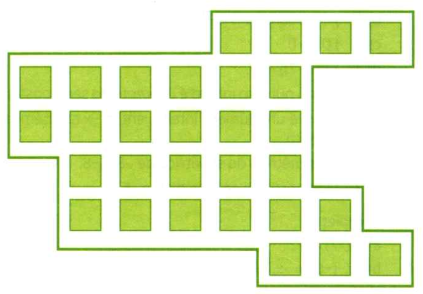
\includegraphics[width=1\linewidth]{6FMA28_imagens/imagem5}
		\end{enumerate}
		$~$ \\ $~$ \\ $~$ \\ $~$ \\ $~$ \\ $~$ \\
	\end{multicols}
\end{document}